\section{Compartment Models}
\begin{frame}{What are Compartmental Models?}
  \begin{itemize}
    \item Mathematical approach for describing and analyzing complex systems
    \item System divided into \textbf{discrete compartments}representing specific states or stages
    \item Transition rates govern the movement of individuals between compartments
    \item They are often applied to modelling of infectious diseases. The population is assigned to compartments with labels \textbf{S}usceptible, \textbf{I}nfectious and \textbf{R}ecovered).
  \end{itemize}
\pause
\vfill
Example of a compartmental model
\begin{center}
    

    \begin{tikzpicture}

  \node[draw, circle, thick, minimum size=1cm, fill=green!15] (S) {S};
  \node[draw, circle, thick, right=1.5cm of S, minimum size=1cm, fill=red!15] (I) {I};
  \node[draw, circle, thick, right=1.5cm of I, minimum size=1cm, fill=blue!15] (R) {R};

  \draw[->] (S) -- node[midway, above] {$\beta$IS} (I);
  \draw[->] (I) -- node[midway, above] {$\gamma$I} (R);

\end{tikzpicture}
\end{center}

\end{frame}

\begin{frame}{Design approach to Compartment Epidemiological Models}
  \begin{itemize}
    \item \textbf{Abstract Models:} 
    \begin{itemize}
      \item \textit{Key question?:} What are general patterns and relationships in epidemics?
      \item \textit{Aims:} Investigate general disease behavior. Explore various modes of transmission and countermeasures
      \item \textit{Characteristics:} High level overview. Models are simple but not trivial. Direct application to real-world situations may be limited, but it still may be a reasonable starting point.
    \end{itemize}

    \pause
    
    \item \textbf{Concrete Models:}
    \begin{itemize}
       \item \textit{Key question?:} What factors are influencing spread of disease in a specific outbreak?
        \item \textit{Aims:} Models detailed information about the situation.
      \item \textit{Characteristics:} Directly relevant to real-world applications. But lessons learned from one epidemic outbreak may not translate to new situations.
     
    \end{itemize}
  \end{itemize}
\end{frame}


\begin{frame}{Abstract and concrete model}

Basic form of SEIR model

\begin{center}
    
\begin{tikzpicture}
  \node[draw, circle, thick, minimum size=1cm, fill=green!15] (S) {S};
  \node[draw, circle, thick, right=1.5cm of S, minimum size=1cm, fill=yellow!15] (E) {E};
  \node[draw, circle, thick, right=1.5cm of E, minimum size=1cm, fill=red!15] (I) {I};
  \node[draw, circle, thick, right=1.5cm of I, minimum size=1cm, fill=blue!15] (R) {R};
   
  \draw[->] (S) -- node[midway, above] {$\beta$IS} (E);
  \draw[->] (E) -- node[midway, above] {$\sigma$E} (I);
  \draw[->] (I) -- node[midway, above] {$\gamma$I} (R);
\end{tikzpicture}
\end{center}

\vfill

Model used in the Czech Republic at early stages of COVID-19 pandemics
  \begin{center}
    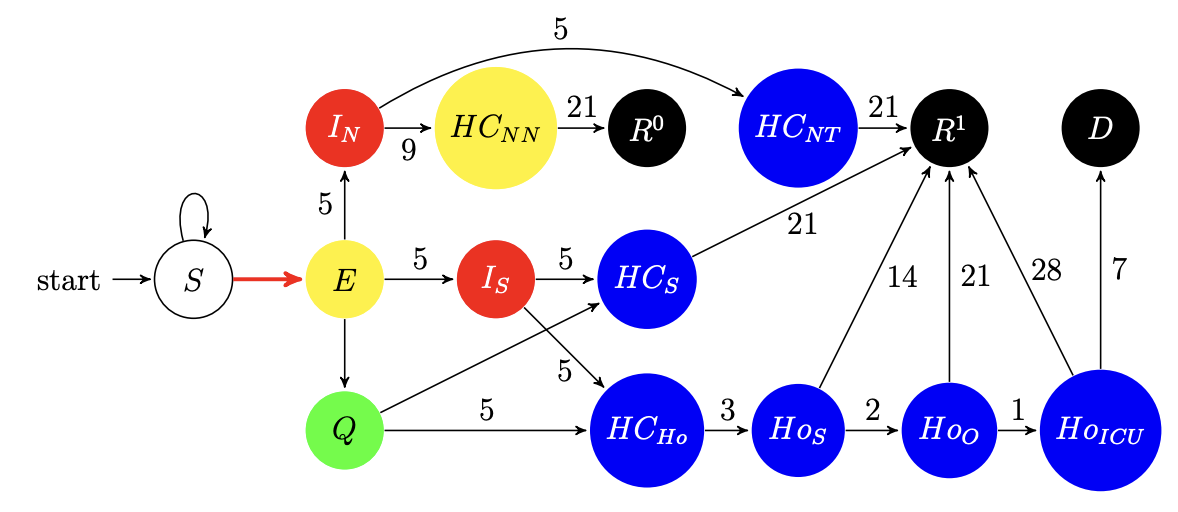
\includegraphics[scale = 0.4]{lesson_3/images/model.png}
  \end{center}
\end{frame}

\subsection{SI Model}
\small
\begin{frame}
  \frametitle{Susceptible-Infected (SI) Model: Overview}
  \begin{itemize}
    \item  The  Susceptible-Infected (SI) model is the simplest form of all disease models. Individuals are born into the simulation with no immunity (susceptible). Once infected and with no treatment, individuals stay infected and infectious throughout their life, and remain in contact with the susceptible population.
    \item Two compartments: Susceptible (S) and Infected (I)
    \item Transition rate: infection rate ($\beta$)
    \item Assumes no recovery or immunity
    \item  Model matches the behavior of diseases like cytomegalovirus 
  \end{itemize}
\end{frame}

\begin{frame}{SI Model: Equations}
  \begin{itemize}
    \item Susceptible (S): Individuals who are not yet infected but can become infected.
    \item Infected (I): Individuals who are infected with the disease.
  \end{itemize}
\vfill
\textbf{Equations:}
  \begin{align*}
    \frac{dS}{dt} &= -\beta S I \\
    \\
    \frac{dI}{dt} &= \beta S I
  \end{align*}

\vfill

\textbf{Diagram:}
  \begin{center}
\begin{tikzpicture}
  \node[draw, circle, thick, minimum size=1cm, fill=green!15] (S) {S};
  \node[draw, circle, thick, right=1.5cm of S, minimum size=1cm, fill=red!15] (I) {I};

  \draw[->] (S) -- node[midway, above] {$\beta$IS} (I);; 
\end{tikzpicture}
  \end{center}
  
\end{frame}


\subsection{SIS Model}
\begin{frame}
  \frametitle{Susceptible-Infected-Susceptible (SIS) Model}
  \begin{itemize}
    \item The Susceptible-Infected-Susceptible (SIS) model extends the SI model by allowing infected individuals to recover and become susceptible again. Assumes no immunity after recovery, allowing for reinfection
    \item  This model is appropriate for diseases that commonly have repeat infections, for example, the common cold (rhinoviruses) or sexually transmitted diseases like gonorrhea or chlamydia
    \item Three states: 
    \begin{itemize}
        \item Susceptible (S): Individuals who are not yet infected but can become infected or have recovered from infection and are susceptible again.
        \item Infected (I): Individuals who are currently infected with the disease.
    \end{itemize}
    \item Epidemic occurs the population reaches an equilibrium between susceptible and infective individuals.
  \end{itemize}
\end{frame}

\begin{frame}{SIS Model: Equations and diagram}
\begin{columns}[t]
\begin{column}{0.5\textwidth}
 \textbf{Transition rates:}
    \begin{itemize}
        \item infection rate ($\beta$) 
        \item  recovery rate ($\gamma$)
    \end{itemize}
        
    \end{column}
    \begin{column}{0.5\textwidth}
    \textbf{Equations:}
          \begin{align*}
            \frac{dS}{dt} &= \gamma I - \beta S I \\
            \\
            \frac{dI}{dt} &= \beta S I - \gamma I
          \end{align*}
    \end{column}
\end{columns}


\vfill
\textbf{Diagram:}
  \begin{center}
\begin{tikzpicture}
  \node[draw, circle, thick, minimum size=1cm, fill=green!15] (S) {S};
  \node[draw, circle, thick, right=1.5cm of S, minimum size=1cm, fill=red!15] (I) {I};

  \draw[->, bend left] (S) to node[midway, above] {$\beta$IS} (I);
  \draw[->, bend left] (I) to node[midway, below] {$\gamma$I} (S);
\end{tikzpicture}
  \end{center}
\end{frame}

\subsection{SI Model with Birth and Death}

\begin{frame}
  \frametitle{SI Model with vital dynamics}
  \begin{itemize}
    \item Extended Susceptible-Infected (SI) model
    \item Compartmental model in epidemiology considering birth and deaths
    \item Two compartments: Susceptible (S) and Infected (I)
    \item Assumes no recovery or immunity
    \item In addition to the simple model, it captures the impact of population dynamics on disease transmission
  \end{itemize}
\end{frame}


\begin{frame}{Equations and model diagram}
\begin{columns}
    \begin{column}{0.5\textwidth}
    \textbf{Transition Rates}
    \begin{itemize}
    \item infection rate ($\beta$)
    \item birth rate ($\upsilon$)
    \item datural death rate ($\mu$)
    \item disease death rate ($\alpha$)
  \end{itemize}
        
    \end{column}
    \begin{column}{0.5\textwidth}
     \textbf{Equations}
  \begin{align*}
    \frac{dS}{dt} &= \upsilon  - \beta S  I - \mu  S \\
    \\
    \frac{dI}{dt} &= \beta  S  I - (\mu + \alpha)  I
  \end{align*}
        
    \end{column}
\end{columns}


\vfill

 \textbf{Model Diagram}
    \begin{center}
\begin{tikzpicture}

  \node[draw, circle, thick, minimum size=1cm, fill=green!15] (S) {S};
  \node[draw, circle, thick, right=1.5cm of S, minimum size=1cm, fill=red!15] (I) {I};
  \node[left=1cm of S] (A) {}; 
  \node[below=1cm of S] (B) {};
  \node[below=1cm of I] (C) {}; 

  \draw[->] (S) -- node[midway, above] {$\beta$IS} (I);
  \draw[->] (A) -- node[midway, above] {$\upsilon$} (S); 
  \draw[->] (S) -- node[midway, right] {$\mu$S} (B); 
  \draw[->] (I) -- node[midway, right] {($\mu$ + $\alpha$)I} (C); 
\end{tikzpicture}
  \end{center}
\end{frame}



\subsection{SIR Model}

\begin{frame}
  \frametitle{Susceptible-Infected-Recovered (SIR) Model: Overview}
  \begin{itemize}
    \item Widely used compartmental model in epidemiology. Assumes individuals gain immunity after recovery
    \item Compartments: Susceptible (S), Infected (I), Recovered (R)

    \item Applications:
      \begin{itemize}
        \item Studying the spread of diseases where recovery and immunity are possible
        \item Evaluating the impact of intervention strategies, such as vaccination or social distancing and predicting the course of an outbreak
      \end{itemize}
  \end{itemize}
\end{frame}

\begin{frame}{SIR Model: Equations and diagram}
\begin{columns}[t]
    \begin{column}{0.5\textwidth}
    \textbf{Transition rates}
     \begin{itemize}
        \item Infection rate ($\beta$)
        \item Recovery rate ($\gamma$)
      \end{itemize}
        
    \end{column}
    \begin{column}{0.5\textwidth}
    \textbf{Equations}
  \begin{align*}
    \frac{dS}{dt} &= -\beta S I \\
    \\
    \frac{dI}{dt} &= \beta S I - \gamma I \\
    \\
    \frac{dR}{dt} &= \gamma I
  \end{align*}
        
    \end{column}
\end{columns}

\vfill
\textbf{Model Diagram}
\begin{center}
\begin{tikzpicture}

  \node[draw, circle, thick, minimum size=1cm, fill=green!15] (S) {S};
  \node[draw, circle, thick, right=1.5cm of S, minimum size=1cm, fill=red!15] (I) {I};
  \node[draw, circle, thick, right=1.5cm of I, minimum size=1cm, fill=blue!15] (R) {R};

  \draw[->] (S) -- node[midway, above] {$\beta$IS} (I);
  \draw[->] (I) -- node[midway, above] {$\gamma$I} (R);

\end{tikzpicture}
  \end{center}
\end{frame}

\begin{frame}{Reproduction Numbers in the SIR Model}
\footnotesize
\begin{columns}
    \begin{column}{0.5\textwidth}
    \textbf{Basic Reproduction Number, \(R_0\)}:
\begin{itemize}
    \item Expected number of cases generated by one case in a population \textbf{where all individuals are susceptible to infection}.
    \item An epidemic will only occur if \(R_0 > 1\).
    \item \(R_0\) \textbf{does not change over the course of an outbreak}, as it is a property of the pathogen and the interaction between the host population and the environment.
    \item Derived from: \(R_0 = \frac{\beta}{\gamma}\) where \(\beta\) is the transmission rate and \(\gamma\) is the recovery rate.
\end{itemize}
    \end{column}

\pause
    \begin{column}{0.5\textwidth}
        \textbf{Effective Reproduction Number, \(R_t\)}:
\begin{itemize}
    \item The number of secondary infections. Not all contacts will become infected and the average number of secondary cases per infectious will be lower than \(R_0\).
    \item \(R_t\) is \textbf{not fixed} and varies over the course of an epidemic due to interventions and immunizations.
    \item When \(R_t\) falls below 1, the outbreak is under control, leading to a decline in new cases.  \(R_t\) 1 means endemic
    \item The calculation of \(R_t\) is  complex  due to changing dynamics.
\end{itemize}
    \end{column}
\end{columns}
\end{frame}

\begin{frame}{Illustration of reproduction number}
\scriptsize
\begin{itemize}
    \item An infected individual (red) can spread the virus among different individuals (black), not reaching part of the population (gray).
    \item Some individuals go into isolation (green), lowering their contagion chance.
    \item  \(R_t\) represents the number of possible new infections caused by a single patient in each outbreak stage.
    \item In the first days, one individual can infect several people before isolation. As the amount of cases gets public awareness and health policies actions helps to control the outbreak, lowering \(R_t\).
\end{itemize}

\begin{center}
        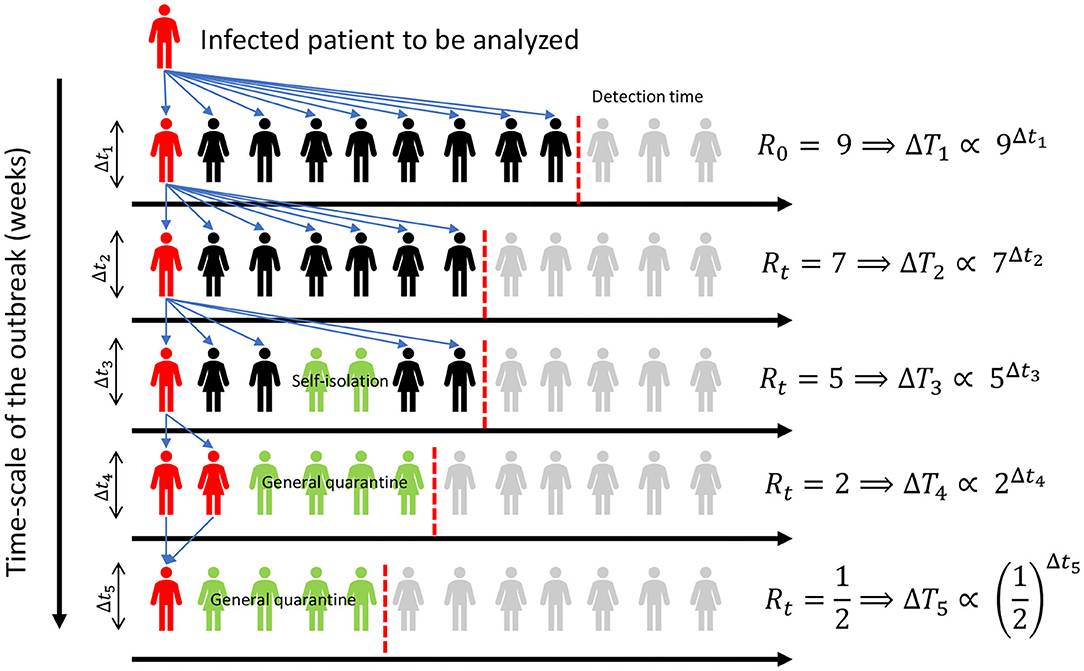
\includegraphics[scale = 0.18]{lesson_3/images/reproductive_number.jpg}
\end{center}
\end{frame}

\begin{frame}{Progress of epidemic by SIR model}
\begin{center}
    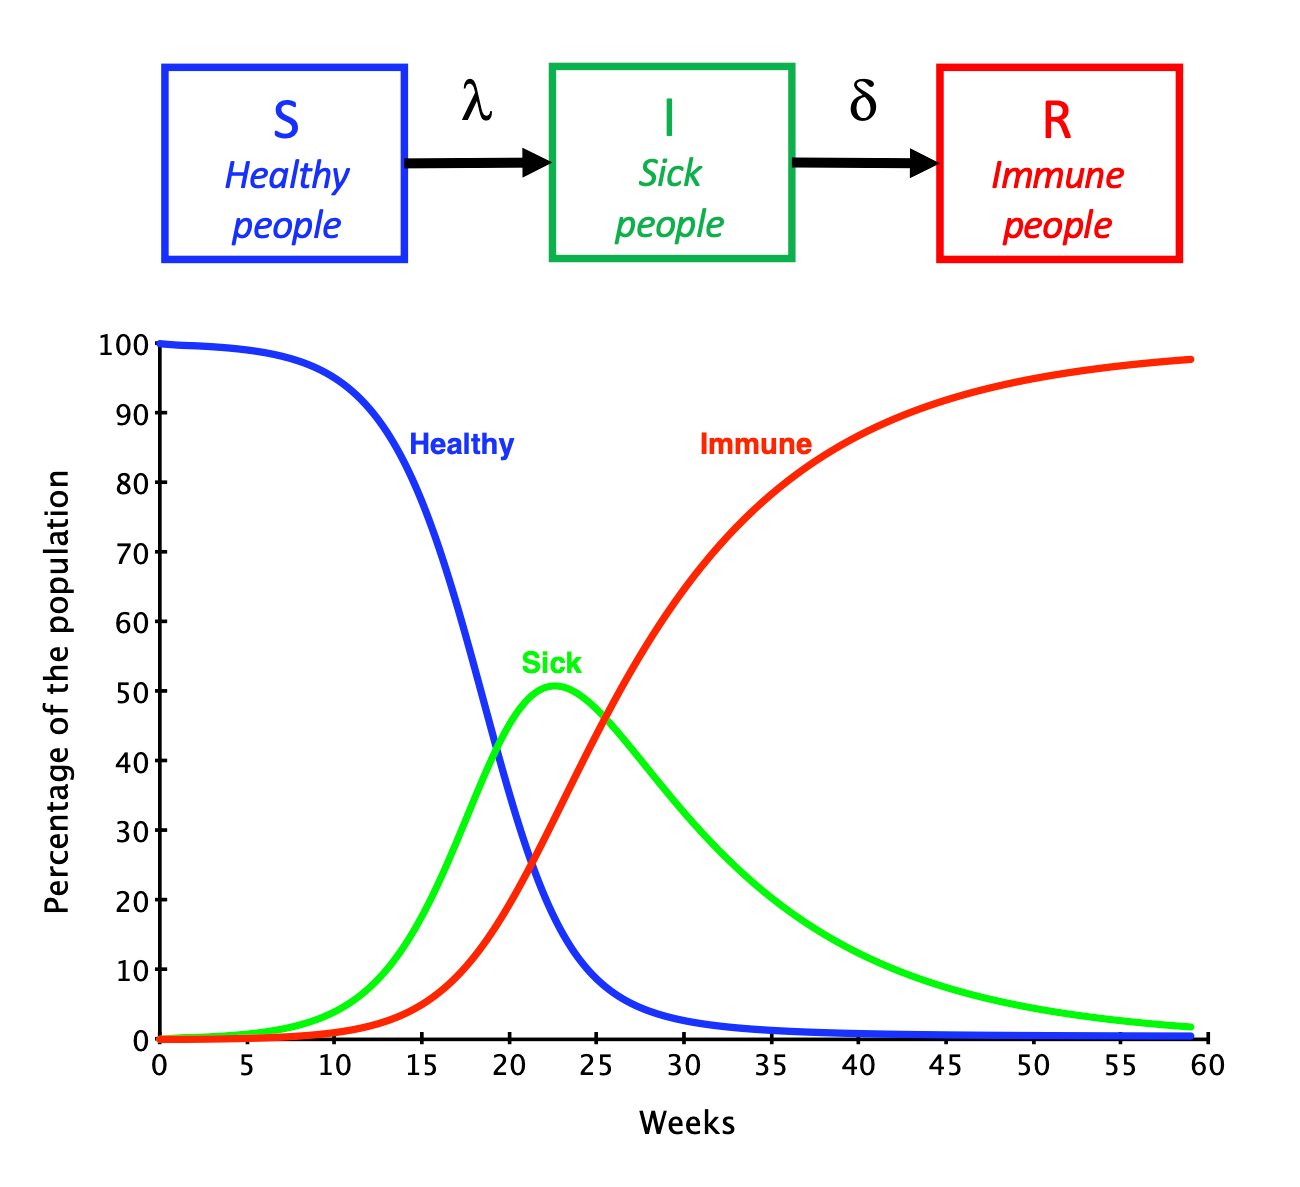
\includegraphics[scale = 0.8]{lesson_3/images/sir_model.png}
\end{center}
    
\end{frame}

\begin{frame}{Epidemic in English boarding school and SIR model}
\begin{center}
    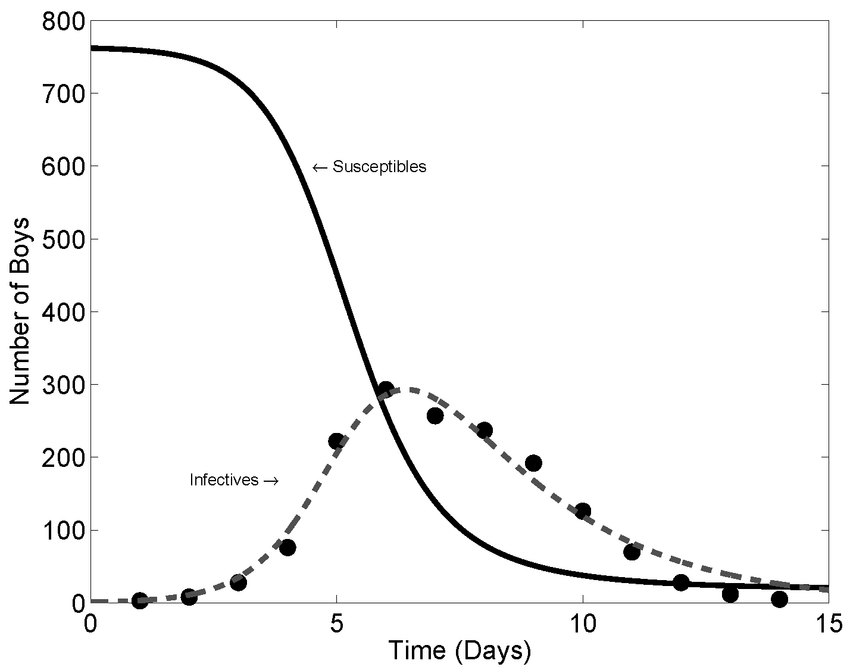
\includegraphics[scale = 0.3]{lesson_3/images/english_boarding_school.png}
\end{center}
    
\end{frame}


\subsection{SEIR Model}

\begin{frame}
  \frametitle{Susceptible-Exposed-Infected-Recovered (SEIR) Model}
  \begin{itemize}
    \item Extended compartmental model in epidemiology. Includes a separate compartment for exposed individuals who are not yet infectious. Suitable for diseases with a latent period where individuals are not infectious immediately after contracting the disease
        
    \item Compartments: Susceptible (S), Exposed (E), Infected (I), Recovered (R)
    \item Exposed individuals (E): have contracted the disease but are not yet infectious; differs from infected individuals (I) who are actively spreading the disease
    \item Applications:
      \begin{itemize}
        \item Studying the spread of diseases with latent periods, such as COVID-19, Ebola, or measles
        \item Evaluating the impact of intervention strategies, such as vaccination or social distancing and predicting the course of an outbreak
      \end{itemize}
  \end{itemize}
\end{frame}


\begin{frame}[t]{SEIR: Model Equations}
\small
\begin{columns}[t]
    \begin{column}{0.5\textwidth}
    \textbf{Rates}
     \begin{itemize}
        \item Infection rate ($\beta$): rate at which susceptible individuals become exposed
        \item Incubation rate ($\sigma$): rate at which exposed individuals become infected
        \item Recovery rate ($\gamma$): rate at which infected individuals recover and gain immunity
  \end{itemize}

    \end{column}
    \begin{column}{0.5\textwidth}
            \textbf{Equations}
    \begin{align*}
    \frac{dS}{dt} &= -\beta S I \\
    \\
    \frac{dE}{dt} &= \beta S I - \sigma E \\
    \\
    \frac{dI}{dt} &= \sigma E - \gamma I \\
    \\
    \frac{dR}{dt} &= \gamma I
  \end{align*}
    \end{column}
\end{columns}  
\vfill
\textbf{Diagram}

\begin{center}
    

\begin{tikzpicture}
  \node[draw, circle, thick, minimum size=1cm, fill=green!15] (S) {S};
  \node[draw, circle, thick, right=1.5cm of S, minimum size=1cm, fill=yellow!15] (E) {E};
  \node[draw, circle, thick, right=1.5cm of E, minimum size=1cm, fill=red!15] (I) {I};
  \node[draw, circle, thick, right=1.5cm of I, minimum size=1cm, fill=blue!15] (R) {R};
   
  \draw[->] (S) -- node[midway, above] {$\beta$IS} (E);
  \draw[->] (E) -- node[midway, above] {$\sigma$E} (I);
  \draw[->] (I) -- node[midway, above] {$\gamma$I} (R);
\end{tikzpicture}
\end{center}
\end{frame}






\begin{frame}
  \frametitle{Applications Beyond Disease Modeling}
  \begin{itemize}
    \item Originally developed for epidemiology, but applicable to other fields with similar dynamics
    \item Key aspects: interacting populations, transitions between states, and time-dependent dynamics
    \item Examples of alternative applications:
      \begin{itemize}
        \item Ecology: predator-prey interactions, invasive species spread
        \item Social networks: spread of information, opinions, or behavior
        \item Computer networks: malware and computer virus propagation
      \end{itemize}
  \end{itemize}
\end{frame}
